% Created by tikzDevice version 0.12.6 on 2024-03-18 22:28:13
% !TEX encoding = UTF-8 Unicode
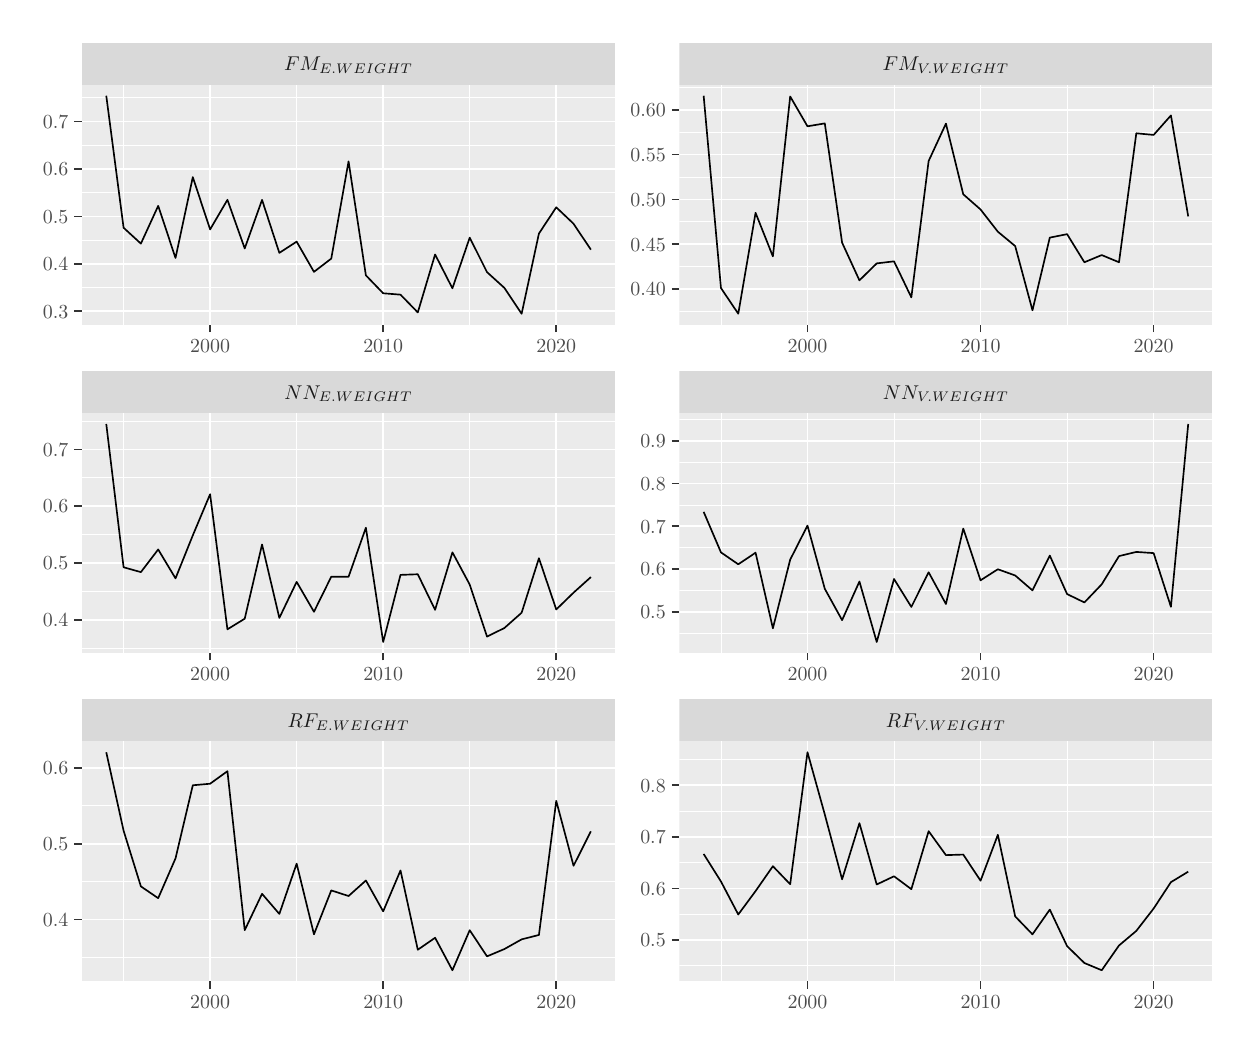
\begin{tikzpicture}[x=1pt,y=1pt]
\definecolor{fillColor}{RGB}{255,255,255}
\path[use as bounding box,fill=fillColor,fill opacity=0.00] (0,0) rectangle (433.62,361.35);
\begin{scope}
\path[clip] (  0.00,  0.00) rectangle (433.62,361.35);
\definecolor{drawColor}{RGB}{255,255,255}
\definecolor{fillColor}{RGB}{255,255,255}

\path[draw=drawColor,line width= 0.6pt,line join=round,line cap=round,fill=fillColor] (  0.00,  0.00) rectangle (433.62,361.35);
\end{scope}
\begin{scope}
\path[clip] ( 19.65,254.04) rectangle (212.26,340.69);
\definecolor{fillColor}{gray}{0.92}

\path[fill=fillColor] ( 19.65,254.04) rectangle (212.26,340.69);
\definecolor{drawColor}{RGB}{255,255,255}

\path[draw=drawColor,line width= 0.3pt,line join=round] ( 19.65,267.42) --
	(212.26,267.42);

\path[draw=drawColor,line width= 0.3pt,line join=round] ( 19.65,284.57) --
	(212.26,284.57);

\path[draw=drawColor,line width= 0.3pt,line join=round] ( 19.65,301.72) --
	(212.26,301.72);

\path[draw=drawColor,line width= 0.3pt,line join=round] ( 19.65,318.87) --
	(212.26,318.87);

\path[draw=drawColor,line width= 0.3pt,line join=round] ( 19.65,336.02) --
	(212.26,336.02);

\path[draw=drawColor,line width= 0.3pt,line join=round] ( 34.66,254.04) --
	( 34.66,340.69);

\path[draw=drawColor,line width= 0.3pt,line join=round] ( 97.19,254.04) --
	( 97.19,340.69);

\path[draw=drawColor,line width= 0.3pt,line join=round] (159.73,254.04) --
	(159.73,340.69);

\path[draw=drawColor,line width= 0.6pt,line join=round] ( 19.65,258.85) --
	(212.26,258.85);

\path[draw=drawColor,line width= 0.6pt,line join=round] ( 19.65,276.00) --
	(212.26,276.00);

\path[draw=drawColor,line width= 0.6pt,line join=round] ( 19.65,293.15) --
	(212.26,293.15);

\path[draw=drawColor,line width= 0.6pt,line join=round] ( 19.65,310.30) --
	(212.26,310.30);

\path[draw=drawColor,line width= 0.6pt,line join=round] ( 19.65,327.45) --
	(212.26,327.45);

\path[draw=drawColor,line width= 0.6pt,line join=round] ( 65.92,254.04) --
	( 65.92,340.69);

\path[draw=drawColor,line width= 0.6pt,line join=round] (128.46,254.04) --
	(128.46,340.69);

\path[draw=drawColor,line width= 0.6pt,line join=round] (191.00,254.04) --
	(191.00,340.69);
\definecolor{drawColor}{RGB}{0,0,0}

\path[draw=drawColor,line width= 0.6pt,line join=round] ( 28.40,336.75) --
	( 34.66,289.05) --
	( 40.91,283.31) --
	( 47.16,296.95) --
	( 53.42,278.14) --
	( 59.67,307.35) --
	( 65.92,288.44) --
	( 72.18,299.14) --
	( 78.43,281.57) --
	( 84.69,299.11) --
	( 90.94,279.97) --
	( 97.19,284.03) --
	(103.45,273.11) --
	(109.70,277.90) --
	(115.95,313.03) --
	(122.21,271.85) --
	(128.46,265.37) --
	(134.72,264.87) --
	(140.97,258.45) --
	(147.22,279.40) --
	(153.48,267.16) --
	(159.73,285.49) --
	(165.98,273.01) --
	(172.24,267.33) --
	(178.49,257.98) --
	(184.74,286.96) --
	(191.00,296.43) --
	(197.25,290.50) --
	(203.51,281.13);
\end{scope}
\begin{scope}
\path[clip] ( 19.65,135.43) rectangle (212.26,222.07);
\definecolor{fillColor}{gray}{0.92}

\path[fill=fillColor] ( 19.65,135.43) rectangle (212.26,222.07);
\definecolor{drawColor}{RGB}{255,255,255}

\path[draw=drawColor,line width= 0.3pt,line join=round] ( 19.65,137.17) --
	(212.26,137.17);

\path[draw=drawColor,line width= 0.3pt,line join=round] ( 19.65,157.68) --
	(212.26,157.68);

\path[draw=drawColor,line width= 0.3pt,line join=round] ( 19.65,178.20) --
	(212.26,178.20);

\path[draw=drawColor,line width= 0.3pt,line join=round] ( 19.65,198.71) --
	(212.26,198.71);

\path[draw=drawColor,line width= 0.3pt,line join=round] ( 19.65,219.23) --
	(212.26,219.23);

\path[draw=drawColor,line width= 0.3pt,line join=round] ( 34.66,135.43) --
	( 34.66,222.07);

\path[draw=drawColor,line width= 0.3pt,line join=round] ( 97.19,135.43) --
	( 97.19,222.07);

\path[draw=drawColor,line width= 0.3pt,line join=round] (159.73,135.43) --
	(159.73,222.07);

\path[draw=drawColor,line width= 0.6pt,line join=round] ( 19.65,147.42) --
	(212.26,147.42);

\path[draw=drawColor,line width= 0.6pt,line join=round] ( 19.65,167.94) --
	(212.26,167.94);

\path[draw=drawColor,line width= 0.6pt,line join=round] ( 19.65,188.46) --
	(212.26,188.46);

\path[draw=drawColor,line width= 0.6pt,line join=round] ( 19.65,208.97) --
	(212.26,208.97);

\path[draw=drawColor,line width= 0.6pt,line join=round] ( 65.92,135.43) --
	( 65.92,222.07);

\path[draw=drawColor,line width= 0.6pt,line join=round] (128.46,135.43) --
	(128.46,222.07);

\path[draw=drawColor,line width= 0.6pt,line join=round] (191.00,135.43) --
	(191.00,222.07);
\definecolor{drawColor}{RGB}{0,0,0}

\path[draw=drawColor,line width= 0.6pt,line join=round] ( 28.40,218.14) --
	( 34.66,166.36) --
	( 40.91,164.61) --
	( 47.16,172.80) --
	( 53.42,162.35) --
	( 59.67,177.89) --
	( 65.92,192.76) --
	( 72.18,143.94) --
	( 78.43,147.78) --
	( 84.69,174.59) --
	( 90.94,148.06) --
	( 97.19,161.09) --
	(103.45,150.29) --
	(109.70,162.94) --
	(115.95,162.93) --
	(122.21,180.66) --
	(128.46,139.36) --
	(134.72,163.61) --
	(140.97,163.84) --
	(147.22,150.98) --
	(153.48,171.76) --
	(159.73,160.12) --
	(165.98,141.32) --
	(172.24,144.40) --
	(178.49,149.94) --
	(184.74,169.62) --
	(191.00,151.11) --
	(197.25,157.19) --
	(203.51,162.82);
\end{scope}
\begin{scope}
\path[clip] ( 19.65, 16.81) rectangle (212.26,103.46);
\definecolor{fillColor}{gray}{0.92}

\path[fill=fillColor] ( 19.65, 16.81) rectangle (212.26,103.46);
\definecolor{drawColor}{RGB}{255,255,255}

\path[draw=drawColor,line width= 0.3pt,line join=round] ( 19.65, 25.40) --
	(212.26, 25.40);

\path[draw=drawColor,line width= 0.3pt,line join=round] ( 19.65, 52.78) --
	(212.26, 52.78);

\path[draw=drawColor,line width= 0.3pt,line join=round] ( 19.65, 80.16) --
	(212.26, 80.16);

\path[draw=drawColor,line width= 0.3pt,line join=round] ( 34.66, 16.81) --
	( 34.66,103.46);

\path[draw=drawColor,line width= 0.3pt,line join=round] ( 97.19, 16.81) --
	( 97.19,103.46);

\path[draw=drawColor,line width= 0.3pt,line join=round] (159.73, 16.81) --
	(159.73,103.46);

\path[draw=drawColor,line width= 0.6pt,line join=round] ( 19.65, 39.09) --
	(212.26, 39.09);

\path[draw=drawColor,line width= 0.6pt,line join=round] ( 19.65, 66.47) --
	(212.26, 66.47);

\path[draw=drawColor,line width= 0.6pt,line join=round] ( 19.65, 93.85) --
	(212.26, 93.85);

\path[draw=drawColor,line width= 0.6pt,line join=round] ( 65.92, 16.81) --
	( 65.92,103.46);

\path[draw=drawColor,line width= 0.6pt,line join=round] (128.46, 16.81) --
	(128.46,103.46);

\path[draw=drawColor,line width= 0.6pt,line join=round] (191.00, 16.81) --
	(191.00,103.46);
\definecolor{drawColor}{RGB}{0,0,0}

\path[draw=drawColor,line width= 0.6pt,line join=round] ( 28.40, 99.52) --
	( 34.66, 71.17) --
	( 40.91, 51.05) --
	( 47.16, 46.79) --
	( 53.42, 61.16) --
	( 59.67, 87.59) --
	( 65.92, 88.15) --
	( 72.18, 92.67) --
	( 78.43, 35.23) --
	( 84.69, 48.37) --
	( 90.94, 41.10) --
	( 97.19, 59.27) --
	(103.45, 33.74) --
	(109.70, 49.60) --
	(115.95, 47.57) --
	(122.21, 53.18) --
	(128.46, 42.03) --
	(134.72, 56.81) --
	(140.97, 28.16) --
	(147.22, 32.48) --
	(153.48, 20.75) --
	(159.73, 35.21) --
	(165.98, 25.77) --
	(172.24, 28.40) --
	(178.49, 31.91) --
	(184.74, 33.50) --
	(191.00, 81.95) --
	(197.25, 58.51) --
	(203.51, 70.95);
\end{scope}
\begin{scope}
\path[clip] (235.51,254.04) rectangle (428.12,340.69);
\definecolor{fillColor}{gray}{0.92}

\path[fill=fillColor] (235.51,254.04) rectangle (428.12,340.69);
\definecolor{drawColor}{RGB}{255,255,255}

\path[draw=drawColor,line width= 0.3pt,line join=round] (235.51,258.79) --
	(428.12,258.79);

\path[draw=drawColor,line width= 0.3pt,line join=round] (235.51,274.98) --
	(428.12,274.98);

\path[draw=drawColor,line width= 0.3pt,line join=round] (235.51,291.18) --
	(428.12,291.18);

\path[draw=drawColor,line width= 0.3pt,line join=round] (235.51,307.37) --
	(428.12,307.37);

\path[draw=drawColor,line width= 0.3pt,line join=round] (235.51,323.57) --
	(428.12,323.57);

\path[draw=drawColor,line width= 0.3pt,line join=round] (235.51,339.76) --
	(428.12,339.76);

\path[draw=drawColor,line width= 0.3pt,line join=round] (250.52,254.04) --
	(250.52,340.69);

\path[draw=drawColor,line width= 0.3pt,line join=round] (313.05,254.04) --
	(313.05,340.69);

\path[draw=drawColor,line width= 0.3pt,line join=round] (375.59,254.04) --
	(375.59,340.69);

\path[draw=drawColor,line width= 0.6pt,line join=round] (235.51,266.89) --
	(428.12,266.89);

\path[draw=drawColor,line width= 0.6pt,line join=round] (235.51,283.08) --
	(428.12,283.08);

\path[draw=drawColor,line width= 0.6pt,line join=round] (235.51,299.28) --
	(428.12,299.28);

\path[draw=drawColor,line width= 0.6pt,line join=round] (235.51,315.47) --
	(428.12,315.47);

\path[draw=drawColor,line width= 0.6pt,line join=round] (235.51,331.67) --
	(428.12,331.67);

\path[draw=drawColor,line width= 0.6pt,line join=round] (281.78,254.04) --
	(281.78,340.69);

\path[draw=drawColor,line width= 0.6pt,line join=round] (344.32,254.04) --
	(344.32,340.69);

\path[draw=drawColor,line width= 0.6pt,line join=round] (406.86,254.04) --
	(406.86,340.69);
\definecolor{drawColor}{RGB}{0,0,0}

\path[draw=drawColor,line width= 0.6pt,line join=round] (244.26,336.75) --
	(250.52,267.26) --
	(256.77,257.98) --
	(263.02,294.44) --
	(269.28,278.69) --
	(275.53,336.48) --
	(281.78,325.71) --
	(288.04,326.75) --
	(294.29,283.66) --
	(300.55,270.04) --
	(306.80,276.17) --
	(313.05,276.91) --
	(319.31,263.89) --
	(325.56,313.17) --
	(331.81,326.67) --
	(338.07,301.14) --
	(344.32,295.65) --
	(350.57,287.62) --
	(356.83,282.43) --
	(363.08,259.22) --
	(369.34,285.49) --
	(375.59,286.73) --
	(381.84,276.58) --
	(388.10,279.18) --
	(394.35,276.58) --
	(400.60,323.18) --
	(406.86,322.59) --
	(413.11,329.63) --
	(419.36,293.15);
\end{scope}
\begin{scope}
\path[clip] (235.51,135.43) rectangle (428.12,222.07);
\definecolor{fillColor}{gray}{0.92}

\path[fill=fillColor] (235.51,135.43) rectangle (428.12,222.07);
\definecolor{drawColor}{RGB}{255,255,255}

\path[draw=drawColor,line width= 0.3pt,line join=round] (235.51,142.61) --
	(428.12,142.61);

\path[draw=drawColor,line width= 0.3pt,line join=round] (235.51,158.03) --
	(428.12,158.03);

\path[draw=drawColor,line width= 0.3pt,line join=round] (235.51,173.46) --
	(428.12,173.46);

\path[draw=drawColor,line width= 0.3pt,line join=round] (235.51,188.88) --
	(428.12,188.88);

\path[draw=drawColor,line width= 0.3pt,line join=round] (235.51,204.30) --
	(428.12,204.30);

\path[draw=drawColor,line width= 0.3pt,line join=round] (235.51,219.73) --
	(428.12,219.73);

\path[draw=drawColor,line width= 0.3pt,line join=round] (250.52,135.43) --
	(250.52,222.07);

\path[draw=drawColor,line width= 0.3pt,line join=round] (313.05,135.43) --
	(313.05,222.07);

\path[draw=drawColor,line width= 0.3pt,line join=round] (375.59,135.43) --
	(375.59,222.07);

\path[draw=drawColor,line width= 0.6pt,line join=round] (235.51,150.32) --
	(428.12,150.32);

\path[draw=drawColor,line width= 0.6pt,line join=round] (235.51,165.75) --
	(428.12,165.75);

\path[draw=drawColor,line width= 0.6pt,line join=round] (235.51,181.17) --
	(428.12,181.17);

\path[draw=drawColor,line width= 0.6pt,line join=round] (235.51,196.59) --
	(428.12,196.59);

\path[draw=drawColor,line width= 0.6pt,line join=round] (235.51,212.02) --
	(428.12,212.02);

\path[draw=drawColor,line width= 0.6pt,line join=round] (281.78,135.43) --
	(281.78,222.07);

\path[draw=drawColor,line width= 0.6pt,line join=round] (344.32,135.43) --
	(344.32,222.07);

\path[draw=drawColor,line width= 0.6pt,line join=round] (406.86,135.43) --
	(406.86,222.07);
\definecolor{drawColor}{RGB}{0,0,0}

\path[draw=drawColor,line width= 0.6pt,line join=round] (244.26,186.39) --
	(250.52,171.74) --
	(256.77,167.44) --
	(263.02,171.63) --
	(269.28,144.31) --
	(275.53,169.11) --
	(281.78,181.43) --
	(288.04,158.58) --
	(294.29,147.26) --
	(300.55,161.23) --
	(306.80,139.36) --
	(313.05,162.13) --
	(319.31,152.03) --
	(325.56,164.55) --
	(331.81,153.09) --
	(338.07,180.33) --
	(344.32,161.65) --
	(350.57,165.65) --
	(356.83,163.40) --
	(363.08,158.01) --
	(369.34,170.60) --
	(375.59,156.68) --
	(381.84,153.65) --
	(388.10,160.20) --
	(394.35,170.40) --
	(400.60,171.91) --
	(406.86,171.48) --
	(413.11,152.08) --
	(419.36,218.14);
\end{scope}
\begin{scope}
\path[clip] (235.51, 16.81) rectangle (428.12,103.46);
\definecolor{fillColor}{gray}{0.92}

\path[fill=fillColor] (235.51, 16.81) rectangle (428.12,103.46);
\definecolor{drawColor}{RGB}{255,255,255}

\path[draw=drawColor,line width= 0.3pt,line join=round] (235.51, 22.37) --
	(428.12, 22.37);

\path[draw=drawColor,line width= 0.3pt,line join=round] (235.51, 41.02) --
	(428.12, 41.02);

\path[draw=drawColor,line width= 0.3pt,line join=round] (235.51, 59.66) --
	(428.12, 59.66);

\path[draw=drawColor,line width= 0.3pt,line join=round] (235.51, 78.31) --
	(428.12, 78.31);

\path[draw=drawColor,line width= 0.3pt,line join=round] (235.51, 96.95) --
	(428.12, 96.95);

\path[draw=drawColor,line width= 0.3pt,line join=round] (250.52, 16.81) --
	(250.52,103.46);

\path[draw=drawColor,line width= 0.3pt,line join=round] (313.05, 16.81) --
	(313.05,103.46);

\path[draw=drawColor,line width= 0.3pt,line join=round] (375.59, 16.81) --
	(375.59,103.46);

\path[draw=drawColor,line width= 0.6pt,line join=round] (235.51, 31.69) --
	(428.12, 31.69);

\path[draw=drawColor,line width= 0.6pt,line join=round] (235.51, 50.34) --
	(428.12, 50.34);

\path[draw=drawColor,line width= 0.6pt,line join=round] (235.51, 68.98) --
	(428.12, 68.98);

\path[draw=drawColor,line width= 0.6pt,line join=round] (235.51, 87.63) --
	(428.12, 87.63);

\path[draw=drawColor,line width= 0.6pt,line join=round] (281.78, 16.81) --
	(281.78,103.46);

\path[draw=drawColor,line width= 0.6pt,line join=round] (344.32, 16.81) --
	(344.32,103.46);

\path[draw=drawColor,line width= 0.6pt,line join=round] (406.86, 16.81) --
	(406.86,103.46);
\definecolor{drawColor}{RGB}{0,0,0}

\path[draw=drawColor,line width= 0.6pt,line join=round] (244.26, 62.77) --
	(250.52, 52.82) --
	(256.77, 40.90) --
	(263.02, 49.35) --
	(269.28, 58.34) --
	(275.53, 51.83) --
	(281.78, 99.52) --
	(288.04, 77.03) --
	(294.29, 53.60) --
	(300.55, 73.90) --
	(306.80, 51.74) --
	(313.05, 54.71) --
	(319.31, 50.05) --
	(325.56, 70.99) --
	(331.81, 62.35) --
	(338.07, 62.55) --
	(344.32, 53.10) --
	(350.57, 69.69) --
	(356.83, 40.21) --
	(363.08, 33.73) --
	(369.34, 42.67) --
	(375.59, 29.46) --
	(381.84, 23.37) --
	(388.10, 20.75) --
	(394.35, 29.70) --
	(400.60, 34.97) --
	(406.86, 43.05) --
	(413.11, 52.58) --
	(419.36, 56.37);
\end{scope}
\begin{scope}
\path[clip] ( 19.65,103.46) rectangle (212.26,118.62);
\definecolor{fillColor}{gray}{0.85}

\path[fill=fillColor] ( 19.65,103.46) rectangle (212.26,118.62);
\definecolor{drawColor}{gray}{0.10}

\node[text=drawColor,anchor=base,inner sep=0pt, outer sep=0pt, scale=  0.72] at (115.95,108.56) {$ RF _{ E.WEIGHT } $};
\end{scope}
\begin{scope}
\path[clip] (235.51,103.46) rectangle (428.12,118.62);
\definecolor{fillColor}{gray}{0.85}

\path[fill=fillColor] (235.51,103.46) rectangle (428.12,118.62);
\definecolor{drawColor}{gray}{0.10}

\node[text=drawColor,anchor=base,inner sep=0pt, outer sep=0pt, scale=  0.72] at (331.81,108.56) {$ RF _{ V.WEIGHT } $};
\end{scope}
\begin{scope}
\path[clip] ( 19.65,222.07) rectangle (212.26,237.23);
\definecolor{fillColor}{gray}{0.85}

\path[fill=fillColor] ( 19.65,222.07) rectangle (212.26,237.23);
\definecolor{drawColor}{gray}{0.10}

\node[text=drawColor,anchor=base,inner sep=0pt, outer sep=0pt, scale=  0.72] at (115.95,227.17) {$ NN _{ E.WEIGHT } $};
\end{scope}
\begin{scope}
\path[clip] (235.51,222.07) rectangle (428.12,237.23);
\definecolor{fillColor}{gray}{0.85}

\path[fill=fillColor] (235.51,222.07) rectangle (428.12,237.23);
\definecolor{drawColor}{gray}{0.10}

\node[text=drawColor,anchor=base,inner sep=0pt, outer sep=0pt, scale=  0.72] at (331.81,227.17) {$ NN _{ V.WEIGHT } $};
\end{scope}
\begin{scope}
\path[clip] ( 19.65,340.69) rectangle (212.26,355.85);
\definecolor{fillColor}{gray}{0.85}

\path[fill=fillColor] ( 19.65,340.69) rectangle (212.26,355.85);
\definecolor{drawColor}{gray}{0.10}

\node[text=drawColor,anchor=base,inner sep=0pt, outer sep=0pt, scale=  0.72] at (115.95,345.79) {$ FM _{ E.WEIGHT } $};
\end{scope}
\begin{scope}
\path[clip] (235.51,340.69) rectangle (428.12,355.85);
\definecolor{fillColor}{gray}{0.85}

\path[fill=fillColor] (235.51,340.69) rectangle (428.12,355.85);
\definecolor{drawColor}{gray}{0.10}

\node[text=drawColor,anchor=base,inner sep=0pt, outer sep=0pt, scale=  0.72] at (331.81,345.79) {$ FM _{ V.WEIGHT } $};
\end{scope}
\begin{scope}
\path[clip] (  0.00,  0.00) rectangle (433.62,361.35);
\definecolor{drawColor}{gray}{0.20}

\path[draw=drawColor,line width= 0.6pt,line join=round] ( 65.92, 14.06) --
	( 65.92, 16.81);

\path[draw=drawColor,line width= 0.6pt,line join=round] (128.46, 14.06) --
	(128.46, 16.81);

\path[draw=drawColor,line width= 0.6pt,line join=round] (191.00, 14.06) --
	(191.00, 16.81);
\end{scope}
\begin{scope}
\path[clip] (  0.00,  0.00) rectangle (433.62,361.35);
\definecolor{drawColor}{gray}{0.30}

\node[text=drawColor,anchor=base,inner sep=0pt, outer sep=0pt, scale=  0.72] at ( 65.92,  6.90) {2000};

\node[text=drawColor,anchor=base,inner sep=0pt, outer sep=0pt, scale=  0.72] at (128.46,  6.90) {2010};

\node[text=drawColor,anchor=base,inner sep=0pt, outer sep=0pt, scale=  0.72] at (191.00,  6.90) {2020};
\end{scope}
\begin{scope}
\path[clip] (  0.00,  0.00) rectangle (433.62,361.35);
\definecolor{drawColor}{gray}{0.20}

\path[draw=drawColor,line width= 0.6pt,line join=round] (281.78, 14.06) --
	(281.78, 16.81);

\path[draw=drawColor,line width= 0.6pt,line join=round] (344.32, 14.06) --
	(344.32, 16.81);

\path[draw=drawColor,line width= 0.6pt,line join=round] (406.86, 14.06) --
	(406.86, 16.81);
\end{scope}
\begin{scope}
\path[clip] (  0.00,  0.00) rectangle (433.62,361.35);
\definecolor{drawColor}{gray}{0.30}

\node[text=drawColor,anchor=base,inner sep=0pt, outer sep=0pt, scale=  0.72] at (281.78,  6.90) {2000};

\node[text=drawColor,anchor=base,inner sep=0pt, outer sep=0pt, scale=  0.72] at (344.32,  6.90) {2010};

\node[text=drawColor,anchor=base,inner sep=0pt, outer sep=0pt, scale=  0.72] at (406.86,  6.90) {2020};
\end{scope}
\begin{scope}
\path[clip] (  0.00,  0.00) rectangle (433.62,361.35);
\definecolor{drawColor}{gray}{0.20}

\path[draw=drawColor,line width= 0.6pt,line join=round] ( 65.92,132.68) --
	( 65.92,135.43);

\path[draw=drawColor,line width= 0.6pt,line join=round] (128.46,132.68) --
	(128.46,135.43);

\path[draw=drawColor,line width= 0.6pt,line join=round] (191.00,132.68) --
	(191.00,135.43);
\end{scope}
\begin{scope}
\path[clip] (  0.00,  0.00) rectangle (433.62,361.35);
\definecolor{drawColor}{gray}{0.30}

\node[text=drawColor,anchor=base,inner sep=0pt, outer sep=0pt, scale=  0.72] at ( 65.92,125.52) {2000};

\node[text=drawColor,anchor=base,inner sep=0pt, outer sep=0pt, scale=  0.72] at (128.46,125.52) {2010};

\node[text=drawColor,anchor=base,inner sep=0pt, outer sep=0pt, scale=  0.72] at (191.00,125.52) {2020};
\end{scope}
\begin{scope}
\path[clip] (  0.00,  0.00) rectangle (433.62,361.35);
\definecolor{drawColor}{gray}{0.20}

\path[draw=drawColor,line width= 0.6pt,line join=round] (281.78,132.68) --
	(281.78,135.43);

\path[draw=drawColor,line width= 0.6pt,line join=round] (344.32,132.68) --
	(344.32,135.43);

\path[draw=drawColor,line width= 0.6pt,line join=round] (406.86,132.68) --
	(406.86,135.43);
\end{scope}
\begin{scope}
\path[clip] (  0.00,  0.00) rectangle (433.62,361.35);
\definecolor{drawColor}{gray}{0.30}

\node[text=drawColor,anchor=base,inner sep=0pt, outer sep=0pt, scale=  0.72] at (281.78,125.52) {2000};

\node[text=drawColor,anchor=base,inner sep=0pt, outer sep=0pt, scale=  0.72] at (344.32,125.52) {2010};

\node[text=drawColor,anchor=base,inner sep=0pt, outer sep=0pt, scale=  0.72] at (406.86,125.52) {2020};
\end{scope}
\begin{scope}
\path[clip] (  0.00,  0.00) rectangle (433.62,361.35);
\definecolor{drawColor}{gray}{0.20}

\path[draw=drawColor,line width= 0.6pt,line join=round] ( 65.92,251.29) --
	( 65.92,254.04);

\path[draw=drawColor,line width= 0.6pt,line join=round] (128.46,251.29) --
	(128.46,254.04);

\path[draw=drawColor,line width= 0.6pt,line join=round] (191.00,251.29) --
	(191.00,254.04);
\end{scope}
\begin{scope}
\path[clip] (  0.00,  0.00) rectangle (433.62,361.35);
\definecolor{drawColor}{gray}{0.30}

\node[text=drawColor,anchor=base,inner sep=0pt, outer sep=0pt, scale=  0.72] at ( 65.92,244.13) {2000};

\node[text=drawColor,anchor=base,inner sep=0pt, outer sep=0pt, scale=  0.72] at (128.46,244.13) {2010};

\node[text=drawColor,anchor=base,inner sep=0pt, outer sep=0pt, scale=  0.72] at (191.00,244.13) {2020};
\end{scope}
\begin{scope}
\path[clip] (  0.00,  0.00) rectangle (433.62,361.35);
\definecolor{drawColor}{gray}{0.20}

\path[draw=drawColor,line width= 0.6pt,line join=round] (281.78,251.29) --
	(281.78,254.04);

\path[draw=drawColor,line width= 0.6pt,line join=round] (344.32,251.29) --
	(344.32,254.04);

\path[draw=drawColor,line width= 0.6pt,line join=round] (406.86,251.29) --
	(406.86,254.04);
\end{scope}
\begin{scope}
\path[clip] (  0.00,  0.00) rectangle (433.62,361.35);
\definecolor{drawColor}{gray}{0.30}

\node[text=drawColor,anchor=base,inner sep=0pt, outer sep=0pt, scale=  0.72] at (281.78,244.13) {2000};

\node[text=drawColor,anchor=base,inner sep=0pt, outer sep=0pt, scale=  0.72] at (344.32,244.13) {2010};

\node[text=drawColor,anchor=base,inner sep=0pt, outer sep=0pt, scale=  0.72] at (406.86,244.13) {2020};
\end{scope}
\begin{scope}
\path[clip] (  0.00,  0.00) rectangle (433.62,361.35);
\definecolor{drawColor}{gray}{0.30}

\node[text=drawColor,anchor=base east,inner sep=0pt, outer sep=0pt, scale=  0.72] at (230.56,264.41) {0.40};

\node[text=drawColor,anchor=base east,inner sep=0pt, outer sep=0pt, scale=  0.72] at (230.56,280.60) {0.45};

\node[text=drawColor,anchor=base east,inner sep=0pt, outer sep=0pt, scale=  0.72] at (230.56,296.80) {0.50};

\node[text=drawColor,anchor=base east,inner sep=0pt, outer sep=0pt, scale=  0.72] at (230.56,312.99) {0.55};

\node[text=drawColor,anchor=base east,inner sep=0pt, outer sep=0pt, scale=  0.72] at (230.56,329.19) {0.60};
\end{scope}
\begin{scope}
\path[clip] (  0.00,  0.00) rectangle (433.62,361.35);
\definecolor{drawColor}{gray}{0.20}

\path[draw=drawColor,line width= 0.6pt,line join=round] (232.76,266.89) --
	(235.51,266.89);

\path[draw=drawColor,line width= 0.6pt,line join=round] (232.76,283.08) --
	(235.51,283.08);

\path[draw=drawColor,line width= 0.6pt,line join=round] (232.76,299.28) --
	(235.51,299.28);

\path[draw=drawColor,line width= 0.6pt,line join=round] (232.76,315.47) --
	(235.51,315.47);

\path[draw=drawColor,line width= 0.6pt,line join=round] (232.76,331.67) --
	(235.51,331.67);
\end{scope}
\begin{scope}
\path[clip] (  0.00,  0.00) rectangle (433.62,361.35);
\definecolor{drawColor}{gray}{0.30}

\node[text=drawColor,anchor=base east,inner sep=0pt, outer sep=0pt, scale=  0.72] at (230.56,147.84) {0.5};

\node[text=drawColor,anchor=base east,inner sep=0pt, outer sep=0pt, scale=  0.72] at (230.56,163.27) {0.6};

\node[text=drawColor,anchor=base east,inner sep=0pt, outer sep=0pt, scale=  0.72] at (230.56,178.69) {0.7};

\node[text=drawColor,anchor=base east,inner sep=0pt, outer sep=0pt, scale=  0.72] at (230.56,194.11) {0.8};

\node[text=drawColor,anchor=base east,inner sep=0pt, outer sep=0pt, scale=  0.72] at (230.56,209.54) {0.9};
\end{scope}
\begin{scope}
\path[clip] (  0.00,  0.00) rectangle (433.62,361.35);
\definecolor{drawColor}{gray}{0.20}

\path[draw=drawColor,line width= 0.6pt,line join=round] (232.76,150.32) --
	(235.51,150.32);

\path[draw=drawColor,line width= 0.6pt,line join=round] (232.76,165.75) --
	(235.51,165.75);

\path[draw=drawColor,line width= 0.6pt,line join=round] (232.76,181.17) --
	(235.51,181.17);

\path[draw=drawColor,line width= 0.6pt,line join=round] (232.76,196.59) --
	(235.51,196.59);

\path[draw=drawColor,line width= 0.6pt,line join=round] (232.76,212.02) --
	(235.51,212.02);
\end{scope}
\begin{scope}
\path[clip] (  0.00,  0.00) rectangle (433.62,361.35);
\definecolor{drawColor}{gray}{0.30}

\node[text=drawColor,anchor=base east,inner sep=0pt, outer sep=0pt, scale=  0.72] at (230.56, 29.22) {0.5};

\node[text=drawColor,anchor=base east,inner sep=0pt, outer sep=0pt, scale=  0.72] at (230.56, 47.86) {0.6};

\node[text=drawColor,anchor=base east,inner sep=0pt, outer sep=0pt, scale=  0.72] at (230.56, 66.50) {0.7};

\node[text=drawColor,anchor=base east,inner sep=0pt, outer sep=0pt, scale=  0.72] at (230.56, 85.15) {0.8};
\end{scope}
\begin{scope}
\path[clip] (  0.00,  0.00) rectangle (433.62,361.35);
\definecolor{drawColor}{gray}{0.20}

\path[draw=drawColor,line width= 0.6pt,line join=round] (232.76, 31.69) --
	(235.51, 31.69);

\path[draw=drawColor,line width= 0.6pt,line join=round] (232.76, 50.34) --
	(235.51, 50.34);

\path[draw=drawColor,line width= 0.6pt,line join=round] (232.76, 68.98) --
	(235.51, 68.98);

\path[draw=drawColor,line width= 0.6pt,line join=round] (232.76, 87.63) --
	(235.51, 87.63);
\end{scope}
\begin{scope}
\path[clip] (  0.00,  0.00) rectangle (433.62,361.35);
\definecolor{drawColor}{gray}{0.30}

\node[text=drawColor,anchor=base east,inner sep=0pt, outer sep=0pt, scale=  0.72] at ( 14.70,256.37) {0.3};

\node[text=drawColor,anchor=base east,inner sep=0pt, outer sep=0pt, scale=  0.72] at ( 14.70,273.52) {0.4};

\node[text=drawColor,anchor=base east,inner sep=0pt, outer sep=0pt, scale=  0.72] at ( 14.70,290.67) {0.5};

\node[text=drawColor,anchor=base east,inner sep=0pt, outer sep=0pt, scale=  0.72] at ( 14.70,307.82) {0.6};

\node[text=drawColor,anchor=base east,inner sep=0pt, outer sep=0pt, scale=  0.72] at ( 14.70,324.97) {0.7};
\end{scope}
\begin{scope}
\path[clip] (  0.00,  0.00) rectangle (433.62,361.35);
\definecolor{drawColor}{gray}{0.20}

\path[draw=drawColor,line width= 0.6pt,line join=round] ( 16.90,258.85) --
	( 19.65,258.85);

\path[draw=drawColor,line width= 0.6pt,line join=round] ( 16.90,276.00) --
	( 19.65,276.00);

\path[draw=drawColor,line width= 0.6pt,line join=round] ( 16.90,293.15) --
	( 19.65,293.15);

\path[draw=drawColor,line width= 0.6pt,line join=round] ( 16.90,310.30) --
	( 19.65,310.30);

\path[draw=drawColor,line width= 0.6pt,line join=round] ( 16.90,327.45) --
	( 19.65,327.45);
\end{scope}
\begin{scope}
\path[clip] (  0.00,  0.00) rectangle (433.62,361.35);
\definecolor{drawColor}{gray}{0.30}

\node[text=drawColor,anchor=base east,inner sep=0pt, outer sep=0pt, scale=  0.72] at ( 14.70,144.94) {0.4};

\node[text=drawColor,anchor=base east,inner sep=0pt, outer sep=0pt, scale=  0.72] at ( 14.70,165.46) {0.5};

\node[text=drawColor,anchor=base east,inner sep=0pt, outer sep=0pt, scale=  0.72] at ( 14.70,185.98) {0.6};

\node[text=drawColor,anchor=base east,inner sep=0pt, outer sep=0pt, scale=  0.72] at ( 14.70,206.49) {0.7};
\end{scope}
\begin{scope}
\path[clip] (  0.00,  0.00) rectangle (433.62,361.35);
\definecolor{drawColor}{gray}{0.20}

\path[draw=drawColor,line width= 0.6pt,line join=round] ( 16.90,147.42) --
	( 19.65,147.42);

\path[draw=drawColor,line width= 0.6pt,line join=round] ( 16.90,167.94) --
	( 19.65,167.94);

\path[draw=drawColor,line width= 0.6pt,line join=round] ( 16.90,188.46) --
	( 19.65,188.46);

\path[draw=drawColor,line width= 0.6pt,line join=round] ( 16.90,208.97) --
	( 19.65,208.97);
\end{scope}
\begin{scope}
\path[clip] (  0.00,  0.00) rectangle (433.62,361.35);
\definecolor{drawColor}{gray}{0.30}

\node[text=drawColor,anchor=base east,inner sep=0pt, outer sep=0pt, scale=  0.72] at ( 14.70, 36.61) {0.4};

\node[text=drawColor,anchor=base east,inner sep=0pt, outer sep=0pt, scale=  0.72] at ( 14.70, 63.99) {0.5};

\node[text=drawColor,anchor=base east,inner sep=0pt, outer sep=0pt, scale=  0.72] at ( 14.70, 91.37) {0.6};
\end{scope}
\begin{scope}
\path[clip] (  0.00,  0.00) rectangle (433.62,361.35);
\definecolor{drawColor}{gray}{0.20}

\path[draw=drawColor,line width= 0.6pt,line join=round] ( 16.90, 39.09) --
	( 19.65, 39.09);

\path[draw=drawColor,line width= 0.6pt,line join=round] ( 16.90, 66.47) --
	( 19.65, 66.47);

\path[draw=drawColor,line width= 0.6pt,line join=round] ( 16.90, 93.85) --
	( 19.65, 93.85);
\end{scope}
\end{tikzpicture}
